\documentclass{article}
\usepackage[left=0.85in, right=0.85in, top=0.5in, bottom=0.95in]{geometry}
\usepackage[T1]{fontenc}
\usepackage[utf8]{inputenc}
\usepackage[italian]{babel}
\usepackage{graphicx}
\usepackage{wrapfig2}
\usepackage{amsmath}
\usepackage{amssymb}
\usepackage{cases}
\usepackage{gensymb} %simboli come ° = \degree  etc etc
\usepackage{subcaption}
\usepackage{hyperref}
\hypersetup{
	colorlinks=true,
	linkcolor=blue,    
	urlcolor=blue,
%	pdfpagemode=FullScreen,
}
\urlstyle{same}
\usepackage{changepage}
\usepackage{lastpage, epstopdf}
\usepackage{fancyhdr}
\usepackage{tcolorbox}
\usepackage{background}
\usepackage{mathtools}
\usepackage{tikz}
\usetikzlibrary{patterns}


%=======HEADER & FOOTER=======%
\def\lesson{Lezione N 3}
\def\outcome{\textbf{Learning Outcomes:} Outcomes go here. }

\pagestyle{fancy}
\fancyhf{}
\renewcommand{\headrulewidth}{0pt}
\renewcommand{\footrulewidth}{1.4pt}
\lfoot{A.M. $\diamond$ \the\year}
\cfoot{\thepage}
\rfoot{\lesson}

%=======CORNELL STYLE FORMAT=======%
\SetBgScale{1}
\SetBgAngle{0}
\SetBgColor{black}
\SetBgContents{\rule{1pt}{0.85\paperheight}}
\SetBgHshift{-1.6in}
\SetBgVshift{-0.1in}

%=======CUSTOM BOXES=======%

\parindent 0ex

%=======BODY=======%
\begin{document}
	\setcounterpageref{secnumdepth}{0}
	\section*{Parte 3} %Date: \hrulefill}
%	\begin{tcolorbox}{\outcome}\end{tcolorbox}

\begin{adjustwidth}{2in}{} 
	
\textbf{{\Large De Saint Venant: Flessione Retta}} \mbox{} \newline
		Si voglia studiare una sollecitazione associata tale che su una faccia la risultante  sia un momento e sull'altra lo stesso momento uguale e opposto: imponendo così una flessione uniforme genero un momento flettente costante su tutta la trave in modo che le fibre trazionate si troveranno in basso e quelle compresse in alto. 
		
\begin{figure}[H]
	\centering
	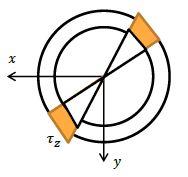
\includegraphics[width=0.5\linewidth]{Immagini/screenshot001}
	\label{fig:screenshot001}
\end{figure}


		Il momento $M_x$ sulla faccia estremale si ottiene così attraverso una determinata distribuzione di pressione, che ipotizzo lungo $z$ essere lineare in $ x $ ed $ y $. 
		
		\[\begin{cases}
			p_x = 0 \\
			p_y = 0 \\
			p_z = a + bx + cy\end{cases} \Rightarrow \begin{cases}
			\tau_{zx} = p_x = 0 \\
			\tau_{zy} = p_y = 0 \\
			\sigma_z = p_z =  a + bx + cy  \\
		\end{cases}  \] 

		Le caratteristiche della sollecitazione sulla $S_l$ saranno:
		\[\begin{matrix}
			\begin{aligned}
				N = \int_A \sigma_zdA = aA + bS_y + cS_x  \hspace{1cm} & M_z = \int_A (\tau_{zy}x -\tau_{zx}y)dA = 0 \\
				T_x = \int_A \tau_{zx}dA = 0 \hspace{1cm} & M_x = \int_A \sigma_zydA = aS_x + bI_{xy} + cI_X \\
				T_y = \int_A \tau_{zy}dA = 0 \hspace{1cm} & M_y = -\int_A \sigma_zxdA = -aS_y - bI_y - cI_{xy}
			\end{aligned}	
		\end{matrix}\]
		Con $S_i$ momento statico, $I_i$ momento d'inerzia, $I_{xy}$ momento centrifugo.
		
		Ottengo in questo modo 3 sollecitazioni distinte ognuna dipendente in modo indipendente dalle altre attraverso un coefficiente di $\sigma_z$. \newline 
		
		Cambiando riferimento in uno baricentrico con assi principali d'inerzia, ottengo l'annullamento di tutti i momenti centrifughi e statici, riconducendomi a sole tre equazioni:
		\[ N = aA \hspace{1cm} M_x = cI_X \hspace{1cm} M_y = - bI_y  \]
		Per avere soltanto sollecitazione flessionale retta e solo un momento lungo la $x$, è necessario annullare i contributi $a$ e $b$, in questo modo, ipotizzando una distribuzione di pressione dipendente solo da $y$ e lineare con essa, si ottiene che: 
		\[\sigma_z = cy\]
		E dunque: 
		\[ N = 0 \hspace{1cm} M_x = cI_X \hspace{1cm} M_y = 0  \]
		L'ipotesi di De Saint Venant per avere flessione retta è quella per cui la distribuzione di tensione ha un andamento lineare lungo la $y$. \newline 
		
		Risolto l'equilibrio esterno si passi ora all'equilibrio interno:
			\[ \begin{cases}
			\begin{aligned}
				\frac{\partial \tau_{zx}}{\partial z} & =0 \\
				
				\frac{\partial \tau_{zy}}{\partial z} & =0 \\
				
				\frac{\partial \tau_{xz}}{\partial x} + \frac{\partial \tau_{yz}}{\partial y} + \frac{\partial\sigma_z}{\partial z} & =0 \\
			\end{aligned}
		\end{cases}\]
		Integrando in $z$ le prime due si ottiene:
		\[\begin{cases}
			\tau_{zx} = cost \\
			\tau_{zy} = cost 
		\end{cases}\]
		All'esterno la pressione indotta non introduce alcuna presenza di tensioni tangenziali, per questo motivo, le tensioni tangenziali oltre che essere costanti, sono anche nulle lungo z. 
		
		Tale risultato, sostituito nella terza equazione, porta a:
		\[ \frac{\partial\sigma_z}{\partial z}  =0\]
		Concludendo che la tensione $\sigma_z$ è costante lungo z. \newline 
		
		Poiché la tensione è nota in $z = l$ ed è quella imposta secondo:
		\[M_x = cI_X \Rightarrow c = \dfrac{M_x}{I_x} \]
		E dalla conoscenza che:
		\[ \sigma_z = cy\]
		Si conclude che: 
		\[ \sigma_z = \dfrac{M_x}{I_x}y \]
		Anche in questo caso, come per lo sforzo normale, ci si riconduce ad uno stato tensionale monoassiale: 
		\[ \left[\begin{array}{ccc}
			0 & 0 & 0 \\
			0 & 0 & 0 \\
			0 & 0 & \dfrac{M_x}{I_x}y
		\end{array}\right]\]
		Ma con la sostanziale differenza che questo è lineare.
		
		Per lo sforzo normale avevo una tensione uniforme sulla sezione e uguale per tutte le sezioni; qui l'andamento rimane sì il medesimo per tutte le sezioni, ma sulla singola sezione la $\sigma_z$ varia sulle $y$ a farfalla, è quindi linearmente dipendente dalla quota $y$, dalla distanza del punto generico $P$ della sezione e dall'asse dei momenti, l'asse rispetto al quale applico il momento flettente, d'altronde per valutare il momento $M_x$ la distanza che si dovrà prendere in considerazione è la $y$. 
		
		Tutti i punti della sezione con la medesima quota $ y $ avranno perciò la stessa tensione $\sigma_z$. 
\newpage		
		La terna principale sarà anche in questo caso formata da $ z $ e due qualsiasi assi
		appartenenti al piano ortogonale a $ z $ e tra loro ortogonali.
		
\begin{figure}[H]
	\centering
	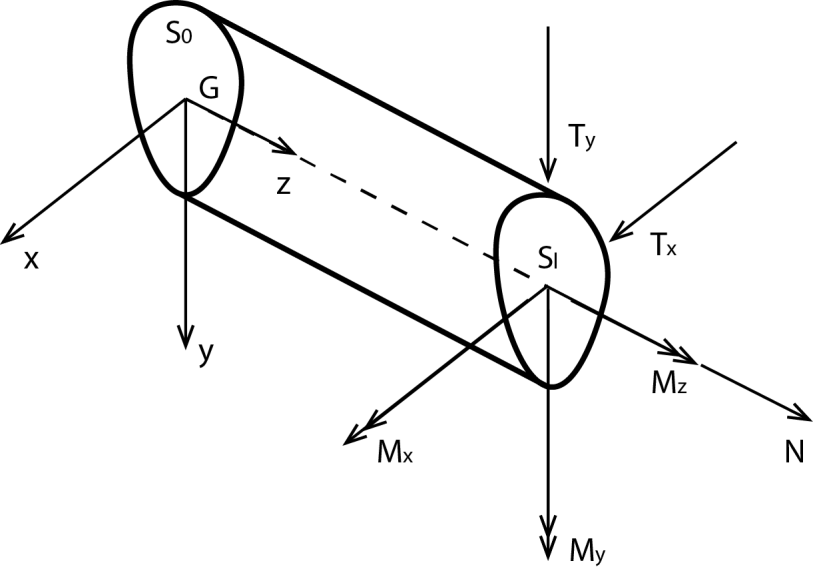
\includegraphics[width=0.5\linewidth]{Immagini/screenshot002}
	\label{fig:screenshot002}
\end{figure}

		Il luogo dei punti caratterizzato da $y=0$ sulla sezione è detto linea o asse neutro delle tensioni, su tutti quei punti la tensioni che agisce è nulla. Tutte queste linee, messe in successione, descrivono un piano, il piano neutro della trave, il luogo dei punti del volume caratterizzato da tensione nulla, completamente scarico. 
		
		In questo caso l'asse neutro coincide con quello baricentrale. \newline
		
		Nel caso di flessione retta, ovvero di quella flessione generata da un momento flettente applicato lungo un asse principale di inerzia, l'asse neutro coincide con l'asse dei momenti. \newline 
		
		Si chiama asse delle sollecitazioni quello perpendicolare a quello dei momenti.
		
		Nel caso di flessione retta, l'asse delle sollecitazioni è perpendicolare all'asse neutro che coincide con quello dei momenti e quello baricentrico. \newline
		
		Al contrario, esistono punti dove la tensione è massima, questi sono altresì caratterizzati dalla massima distanza dall'asse baricentrico $x$; in termini di modulo, sarà il punto più lontano da tale asse ad essere il più sollecitato, a trazione o compressione. \newline
		
		\item[!!] È importante notare che un grafico a farfalla siffatto NON è la reale rappresentazione del momento su $z$, questo uscente/ortogonale dal piano del foglio/sezione, ma riporta soltanto L'ANDAMENTO del modulo del vettore $|\sigma_z|$. 
		
		\item[!!] A seguito di un $M_x$ positivo, si viene a formare sulla sezione una parte di trave sollecitata a ~ $  \underset{+}{trazione} $ e un'altra sollecitata a ~ $ \underset{-}{compressione} $.

		Alla massima distanza tra un massimo ed un minimo avrò, in termini di modulo, il momento massimo. 

		Tra le infinite soluzioni equilibrate, l’unica
		congruente sarà data dalla risoluzione delle seguenti equazioni di Navier:
			\[ 
		\begin{cases}
			\begin{aligned}
				\varepsilon_{xx} =   \frac{\partial u_x}{\partial x} = \dfrac{1}{E}[\sigma_x - \nu(\sigma_y + \sigma_z)] = -\dfrac{\nu M_x}{EI_x}y \\
				\varepsilon_{yy} =   \frac{\partial u_y}{\partial y} = \dfrac{1}{E}[\sigma_y - \nu(\sigma_x + \sigma_z)] = -\dfrac{\nu M_x}{EI_x}y \\
				\varepsilon_{zz} =   \frac{\partial u_z}{\partial z} = \dfrac{1}{E}[\sigma_z - \nu(\sigma_x + \sigma_y)] = \dfrac{M_x}{EI_x}y\\
			\end{aligned}
		\end{cases} \hspace{1cm} \begin{cases}
			\begin{aligned}
				\gamma_{xy} =   \frac{\partial u_y}{\partial x} + \frac{\partial u_x}{\partial y} = \dfrac{1}{G} \tau_{xy} = 0\\
				\gamma_{yz} =   \frac{\partial u_y}{\partial z} + \frac{\partial u_z}{\partial y} = \dfrac{1}{G} \tau_{xz} = 0 \\
				\gamma_{zx} =   \frac{\partial u_z}{\partial x} + \frac{\partial u_x}{\partial z} = \dfrac{1}{G} \tau_{yz} = 0 \\
			\end{aligned}
		\end{cases}
		\]
		Ecco il risultato: l'allungamento su $z$ è quello responsabile delle fibre tese e compresse in \textit{meccanica dei solidi}: tanto è maggiore l'allungamento quanto sarà maggiore la distanza $y$.
		\[\begin{cases}
			y>0 ~ \text{allungamento} \\
			y<0 ~\text{accorciamento}
		\end{cases}\]

\begin{figure}
	\centering
	\begin{tikzpicture} [>=latex]
		%\draw [help lines] (0,0) grid (6,6);
		\draw[thick] (0,0) rectangle (4, 2);
		\draw[thick, green] (-1,0.25) -- (1,2) -- (3,2) -- (5, 0.25);
		\draw[thick, green] (5,0.25) arc (0:-180:3 and 0.5);
		\draw[ ->, thick] (5.5,0.25) arc (0:45:0.5 and 2);
		\draw[ ->, thick] (-1.5,0.25) arc (180:135:0.5 and 2);		
	\end{tikzpicture}
\end{figure}
		
		Integrando le relazioni così ottenute da Navier ottengo gli spostamenti, questi sono definiti a meno di 3 funzioni di integrazione che non posso ignorare a priori a meno che non descrivano un moto rigido, infatti questo per definizione non concorrerà allo stato tensionale e deformativo della trave.
		\[ \begin{cases}
			\begin{aligned}
				u & = -\dfrac{\nu M_x}{EI_x}yx + u_0(z,y) \\
				v & = -\dfrac{1}{2}\dfrac{\nu M_x}{EI_x}y^2 + v_0(z,x) \\
				w & = \dfrac{M_x}{EI_x}yz + w_0(x,y)
			\end{aligned}
		\end{cases} \]
		Sostituisco le $ u_0,  v_0,  w_0$ incognite nella formulazione dello scorrimento $xt$, e in questo caso differentemente dallo sforzo normale, si ottiene:
		\[ 	\gamma_{xy} =   \frac{\partial u}{\partial y} + \dfrac{\partial v}{\partial x} = -\dfrac{\nu M_x}{EI_x}x + \dfrac{\partial u_0(z,y)}{\partial y} + dfrac{\partial v_0(z,x)}{\partial x} = 0\] 
		Derivando rispetto ad $x$:
		\[  \dfrac{\partial^2 v_0(z,x)}{\partial x^2} = \dfrac{\nu M_x}{EI_x}  \]
		Integrando due volte rispetto ad $x$:
		\[  v_0 = \dfrac{1}{2}\dfrac{\nu M_x}{EI_x}x^2 + \underbrace{xv'_0(z) + v'_1(z)}_\text{$v_1(x,z)$} \]
		E quindi si giunge a: 
		\[ \begin{cases}
			\begin{aligned}
				u & = -\dfrac{\nu M_x}{EI_x}yx + u_0(z,y) \\
				v & = \dfrac{1}{2}\dfrac{\nu M_x}{EI_x}(x^2 - y^2) + v_1(x,z) \\
				w & = \dfrac{M_x}{EI_x}yz + w_0(x,y)
			\end{aligned}
		\end{cases} \]
		La nuova terna di spostamenti però non descrive ancora un moto rigido:
		\[\gamma_{yz} =   \frac{\partial v}{\partial z} + \frac{\partial w}{\partial y} = \dfrac{\partial v_1(x,z)}{\partial z} + \dfrac{M_x}{EI_x}z +\dfrac{\partial w_0(x,y)}{\partial y} = 0\]
		Similmente a poco sopra derivo rispetto a $z$ ed integro due volte rispetto a $z$: 
		\[  \dfrac{\partial^2 v_1(x,z)}{\partial z^2} = - \dfrac{M_x}{EI_x}  \]
		\[  v_1 = -\dfrac{1}{2}\dfrac{M_x}{EI_x}z^2 + v_2(x,z) \]
		Ora le funzioni $ u_0,  v_2,  w_0$ descrivono un moto rigido: le deformazioni ad esse associate sono nulle:
		\[\begin{cases}
			\begin{aligned}
				\gamma_{xy} =   \frac{\partial v}{\partial x} + \frac{\partial u}{\partial y} = \dfrac{\nu M_x}{EI_x}x - \dfrac{\nu M_x}{EI_x}x  = 0\\
				\gamma_{yz} =   \frac{\partial v}{\partial z} + \frac{\partial w}{\partial y} = + \dfrac{M_x}{EI_x}z + \dfrac{M_x}{EI_x}z = 0 \\
				\gamma_{zx} =   \frac{\partial u_z}{\partial x} + \frac{\partial u_x}{\partial z} = 0 \\
			\end{aligned}\end{cases}\]
		
		 E quindi le rispettive funzioni sono eliminabili dalla soluzione finale, che in questo modo sarà:
		\[\boxed{\begin{dcases}			
				u & = -\dfrac{\nu M_x}{EI_x}yx + u_0(z,y) \\
				v & = -\dfrac{1}{2}\dfrac{\nu M_x}{EI_x}(x^2 - y^2)  -\dfrac{1}{2}\dfrac{ M_x}{EI_x}z^2 \\
				w & = \dfrac{M_x}{EI_x}yz + w_0(x,y)	
		\end{dcases}} \]
		
		La linea d'asse (l'asse baricentrico) si trova sostituendo $x=y=0$, lo spostamento ad essa associato è:
		\[ v  = -\dfrac{1}{2}\dfrac{ M_x}{EI_x}z^2 \] 
		Quadratico rispetto a $z$, il che significa che la linea d'asse non subisce spostamenti $u$ sul piano della sezione e quindi lungo l'asse dei momenti; non subisce neanche allungamenti $w$, ma subisce solamente degli spostamenti $v$ ortogonali al sua asse e a quello dei momenti. \newline 
		
		Se si rappresenta la trave in un piano $xy$, la linea d'asse, a seguito di un momento $M_x$ si inflette nel modo seguente, subendo solo spostamenti in direzione $y$:
		
\begin{figure}[H]
	\centering
	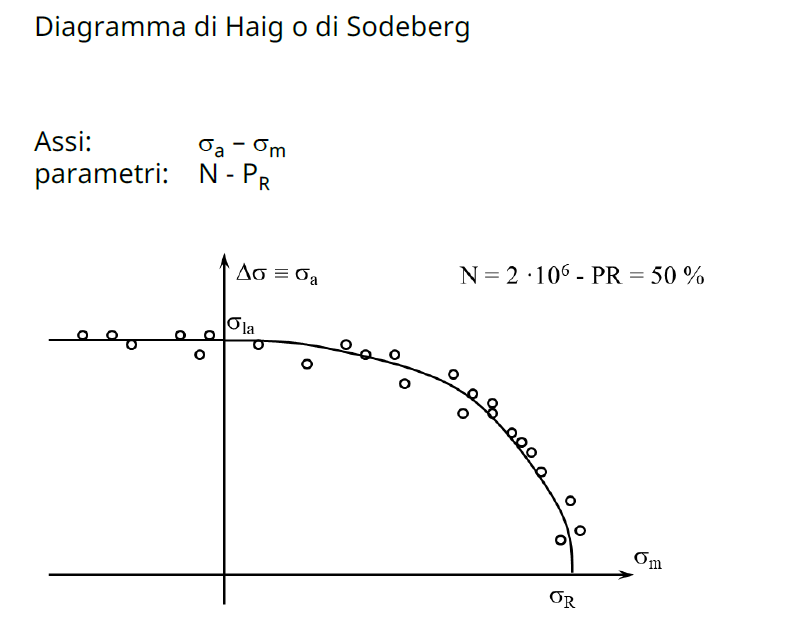
\includegraphics[width=0.5\linewidth]{Immagini/screenshot003}
	\label{fig:screenshot003}
\end{figure}

		La linea d'asse rimane perciò in un piano chiamato piano di inflessione, ortogonale questo all'asse dei momenti, in questo caso $yz$. \newline 
		
		Si valuti adesso rotazione e curvatura dell'andamento quadratico. 
		\[ \chi = \dfrac{1}{R} = \dfrac{\ddot{v}}{(1+\dot{v}^2)^{3/2}}\]
		Dove $v$ è l'abbassamento. Inoltre, sotto le ipotesi di piccoli spostamenti e di Bernoulli, per la quale le sezioni rette continuano ad essere rette per ogni sollecitazione applicata $\dot{v}\approx 0$ e dunque: 
		\[ \chi = \dfrac{1}{R} = \ddot{v} = \dfrac{ M_x}{EI_x} \]
		Essendo la curvatura costante in $z$, la deformata d'asse sarà a curvatura costante, inoltre, come non notare che la curvatura dipende dal momento stesso $M_x$ e dal modulo di rigidezze flessionale $EI_x$? Tanto maggiore sarà quest'ultimo, infatti, tanto maggiore sarà il raggio di curvatura e tanto minore sarà la curvatura: Maggiore sarà $EI_x$ minore sarà la deformabilità della trave a flessione. \newline 
		
		A parità di momento flettente, per avere piccole deformate flessionali o scelgo un materiale più rigido o scelgo una sezione maggiore, la sezione della trave è d'altro canto legata al momento d'inerzia, che ad esempio, per trave a sezione quadrata:
		\[ I= \dfrac{bh^3 }{12}\]
		Con $b,h$ dimensioni della sezione. \newline 
		
		Ma se fossi in grado di realizzare la stessa inerzia on meno materiale? Sarebbe auspicabile, meno peso, meno ingombro e meno costo \dots 
		
		Dalla definizione, il momento d'inerzia vale: 
		\[  I_x = \int_A y^2dA\]
		Infatti questo non dipende da come è distribuito il materiale rispetto all'asse $x$ ma solo da com'è distribuito intorno all'asse $y$. 
		
		Se la stessa quantità di materiale  si riesce a distribuire il più lontano possibile dall'asse $ x $ e quindi a maggiori quote $y$, ottengo di fatto un maggiore momento d'inerzia. 
		
\begin{figure}
	\centering
	\begin{tikzpicture} [>=latex]
		%\draw [thin, help lines] (0,0) grid (10,10);
		\draw[thick] (0,0) rectangle (4, 1);
		\draw[thick] (1.5,1) rectangle (2.5, 4);
		\draw[thick] (0,4) rectangle (4, 5);
		\draw[pattern=north east lines, thick] (0,1) rectangle (1.5, 4);
		\draw[pattern=north east lines, thick] (2.5,1) rectangle (4, 4);
		\draw[->>, thick, red] (2, 5) -- (2, -1) node [pos=1, below] {$M_y$};
		\draw[->, thick] (-0.5, 2.5) -- (4.5, 2.5) node [pos=1, right] {$z$};
		\draw[->, thick] (-0.5, 2.5) -- (-0.5, 1) node [pos=1, below] {$y$};
		\draw[->, thick] (-0.5, 2.5) -- (-2, 1.5) node [pos=1, below] {$z$};
		\draw[->>, thick, blue] (-0.5, 2.5) -- (-2, 2.5) node [pos=1, left] {$M_x$};
	\end{tikzpicture}
\end{figure}

		\item[!!] Le stessa sezione però, sollecitata secondo l'asse di un momento $M_y$ non potrebbe comportarsi allo stesso modo, infatti in questo caso è importante  che dipenderà questo dalla distanza a cui è collocato il materiale lungo $x$, in questo  lungo $x$ c'è molta distribuzione di materiale il che comporterà $I_y$ avere un ODG inferiore, ma in cosa si traduce un ODG inferiore sul momento d'inerzia? Ad un ODG superiore sulle tensioni! \newline 
		
		Ritornano alla linea d'asse, si è più che dimostrato come questa non subisca deformazioni ma solo spostamenti: quando applico un'inflessione alla linea d'asse questa per ogni punto in configurazione deformata deve avere la stessa quota $z$ d'altronde vale $w=0$, le sezioni si trovano perciò alla stessa quota $z$ senza allungamenti; la linea d'asse però inflettendosi ha fatto però un percorso ben più lungo perché per arrivare alla stessa quota con una traiettoria curva si vuole un cammino maggiore, mi aspetto allora un allungamento $\varepsilon_{zz}$ che però non c'è, sostituisco allora l'equazione dell'asse baricentrico nello spostamento $w$, ma questo continua ad essere nullo. \newline 
		
		Tale paradosso è giustificato dai piccoli spostamenti, infatti posso scrivere lo spostamento che compie l'asse come somma in quadratura:
		\[ ds^2 \approx dz^2 + dv^2 = dz^2 + \left[\dfrac{M_x}{EI_x}zdz\right]^2 = dz^2 \left[1+ \left(\dfrac{M_xz}{EI_x}\right)^2\right] \]
		Per piccoli spostamenti, che sono quelli con cui lavoriamo:
		\[\left(\dfrac{M_xz}{EI_x}\right)^2 << 1\]
		E quindi si può trascurare:
		\[  ds^2 \approx dz^2 \]
		Nell’ipotesi di piccole deformazioni la lunghezza dell’asse può essere considerata costante. \newline
		
		All'infuori della linea d'asse le fibre si allungano, ciò che si ottiene è perciò una funzione di allungamento/spostamento su $z$ che dipende da $y$:
		\[ z' = z + w = z + \dfrac{M_x}{EI_x}yz = K \left(1-\dfrac{y}{R}\right)\]
		Tanto più ci si sposta lungo la $y$ tanto più le fibre si allungano. 
		
		La sezione subisce così degli spostamenti $w$ proporzionali alla quota $y$, tale spostamento non fa nient'altro che generare una rotazione rigida della sezione che ruoterà a seguito della flessione intorno all'asse dei momenti, dalla definizione la rotazione è data da: 
		\[  \varphi = -\dfrac{ \partial v}{ \partial z}\]
		
\begin{figure}[H]
	\centering
	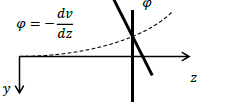
\includegraphics[width=0.5\linewidth]{Immagini/screenshot004}
	\label{fig:screenshot004}
\end{figure}


		Una sezione retta che giace su un piano ortogonale alla linea d’asse, una volta deformata
		continua a giacere su un piano che è ruotato ma che è ancora ortogonale alla linea d’asse (ora
		deformata) e dunque: 
		\[ \varphi(z) = \dfrac{M_x}{EI_x}z \]
		Oppure, equivalentemente, se si considera che lo spostamento $z'$ porta la sezione su un piano ortogonale al piano contenente la deformata della linea d’asse
		la cui traccia sul piano $ yz $ è una retta che passa per il centro del raggio osculatore:
		\[ d\varphi(z) = \dfrac{1}{|R|}ds = \dfrac{M_x}{EI_x}dz \]
		
		All'estremo della trave si ottengono gli stessi valori incontrati in \textit{meccanica dei solidi} della trave a mensola sollecitata con un momento:
		\[ v(l) = -\dfrac{1}{2}\dfrac{M_x}{EI_x}l^2 \hspace{1cm} \varphi(l) = \dfrac{M_x}{EI_x}l\]
		
		Cosa accade ora nella sezione della trave a seguito della flessione? 
		
		A seguito della deformazione associata alla flessione i segmenti rettilinei e paralleli ad $x$ si trasformano in archi di circonferenza il: segmento si inflette secondo una curvatura che abbiamo imparato a riconoscere costante, ottenendo la seguente mappatura della sezione.
		
\begin{figure}[H]
	\centering
	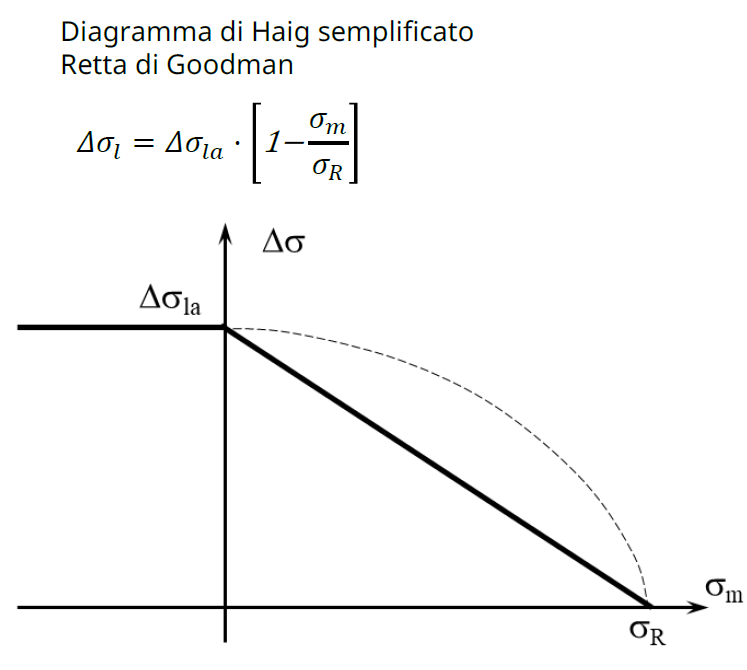
\includegraphics[width=0.5\linewidth]{Immagini/screenshot005}
	\label{fig:screenshot005}
\end{figure}

		La sezione resta piana ma varia la sua forma: ricordando che per le $y>0$ la tensione è di trazione, cosa accade alle fibre della trave? Quelle che si allungano assialmente si avvicinano tra loro, quelle che si comprimono si allontanano tra loro: questo è un meccanismo del materiale per compensare la variazione di volume, le fibre trazionate si avvicinano tra loro occupando meno volume mentre quelle compresse accorciandosi si allontanano tra di loro per occupare più volume.
		
		D'altro canto in una sollecitazione flessionale la deformazione è associata ad una variazione di volume nulla, a differenza della trazione dove caratterizzata da strizione e dunque da una diminuzione di volume. \newline 
		
		In condizioni statiche si ha il bisogno di rispondere principalmente a due domande: 
		\begin{enumerate}
			\item l'oggetto resiste? La tensione che si instaura a seguito delle azioni esterne è minore di quella massima che il materiale può sopportare?
			\item l'oggetto continua a funzionare? È garantita la funzionalità?
		\end{enumerate}
		Se la seconda domanda si traduce nei termini di freccia massima contenuta entro un certo dato da una normativa, alla prima domanda è più articolato rispondere perché implica un confronto tra scalari:
		\[ |\sigma(P)|\leq \sigma_{amm}\]
		Devo quindi tradurre il tensore delle tensioni in una tensione equivalente monodimensionale $\sigma(P)$, e non sempre è immediato. 
		\[\sigma_{amm} = \dfrac{\sigma_{lim}}{X}\]
		Invece tiene conto del fatto che per dimensionare un oggetto che lavorerà in un campo applicativo reale l'effettiva resistenza del materiale sarà ben diversa da quelle studiate in condizioni simil-ideali di laboratorio, è ovvio che si lavorerà con una tensione più bassa data da un opportuno coefficiente di sicurezza normato. È logico poi che in condizioni di operatività può subire delle modifiche, sarà dunque necessario programmare manutenzioni e rilievi per constatare che le opportune e reali condizioni di carico rientrino nelle tensioni ammissibili (e quindi quelle limite ridotte) calcolate in fase di progetto. \newline 
		
		In più, poiché nelle applicazioni strutturali/meccaniche è sempre bene lavorare in campo elastico e non in campo plastico, la tensione limite di cui si dovrà tenere conto in fase di progetto sarà quella di snervamento. \newline 
		
		Ritornando alla definizione del $ \sigma(P) $, nei casi analizzati di sforzo normale e di flessione retta siano in condizioni auspicabili perché entrambe contribuiscono con uno sforzo monodimensionale, è facile dimostrare quindi che per lo sforzo normale in fase di progettazione non sarà tanto importante la forma, ma la sezione dell'oggetto: 
		\[ \sigma_z = \dfrac{N}{A} \leq \sigma_{amm} \Rightarrow A \geq \dfrac{N}{\sigma_{amm}}\]
		Per la flessione retta invece dovrà sussistere la relazione: 
		\[ \sigma_z = \dfrac{M_x}{I_x}y \leq \sigma_{amm} \]
		Noto l'andamento della tensione so che: punti alla stessa quota $y$ hanno tutti lo stesso valore di tensione; ogni sezione presenta esattamente lo stesso andamento; i punti maggiormente sollecitati saranno quelli a massima/minima distanza $y$, tutto ciò porta così ad effettuare due verifiche in dipendenza del materiale utilizzato. 
		
\begin{figure}[H]
	\centering
	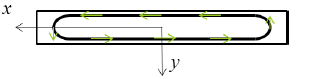
\includegraphics[width=0.5\linewidth]{Immagini/screenshot006}
	\label{fig:screenshot006}
\end{figure}
		
		Il materiale è isotropo e si comporta a trazione e compressione nello stesso modo (ex acciaio)? Utilizzerò allora tra i due il massimo del valore assoluto dei due punti maggiormente sollecitati:
		\[ \sigma_z(P_1) = \dfrac{M_x}{I_x/h_1} \hspace{1cm} \sigma_z(P_2) = \dfrac{M_x}{I_x/h_2}\]
		\[ \max{|\sigma_z(P_1)|; |\sigma_z(P_2)|}\]
		
		Il materiale si comporta in maniera diversa a trazione e compressione (ex ghisa, ceramica, calcestruzzo)? Utilizzerò dei valori specifici ottenuti a trazione o compressione, a seconda di come il materiale lavorerà. \newline 
		
		Ciò che poi in fase di progettazione andrà massimizzato sarà proprio il denominatore di siffatta tensione, condensato nel modulo di resistenza a flessione:
		\[w_x = \dfrac{I_x}{y}\]
		È il rapporto tra l'inerzia e la quota massima di distanza dall'asse baricentrico, e per questo che in fase di progetto è necessario scegliere una sezione che massimizzi l'inerzia e ponga il più lontano possibile dall'asse $x$ il materiale, in questo modo sarà maggiore l'inerzia sull'asse $ x $ e minore la tensione sulla trave.
		
	\newpage
	{\Large \textbf{NOTE}}
%	\vfill
%\begin{tcolorbox}[height=4.5cm]
%	This box has a height of 4.5cm.
%\end{tcolorbox}

%DA DECOMMENTARE PER AVERE LA VERSIONE STAMPABILE A DUE PAGINE 	
%	\newpage
%		\null
%		\vfill
%\begin{tcolorbox}[height=4.5cm]
%	This box has a height of 4.5cm.
%\end{tcolorbox}
%		
\end{adjustwidth}
\end{document}